\documentclass{article}
%\documentclass{IEEETran}

%\usepackage{anysize}
%\usepackage[left=1.9cm,right=1.9cm,top=2.54cm,bottom=1.9cm]{geometry}
%\usepackage{sectsty}
%\sectionfont{\normalsize \bf}
%\subsectionfont{\normalsize \bf}

%\IEEEoverridecommandlockouts  
%\overrideIEEEmargins

%\usepackage{siunitx}
\usepackage{setspace} 
%\doublespacing
\usepackage{cite}
\usepackage{amsmath}
\usepackage{amsthm}
\theoremstyle{remark}
\newtheorem{assumption}{Assumption}
\usepackage{graphicx}
\usepackage{fancyhdr}
\usepackage[bottom]{footmisc}
% \usepackage{hyperref}
\usepackage[pdfusetitle]{hyperref}
\usepackage{amssymb}
\usepackage{enumerate}
\usepackage{mathtools}

\usepackage{ifthen}
\DeclarePairedDelimiter{\norm}{\lVert}{\rVert}
\DeclarePairedDelimiter\abs{\lvert}{\rvert}%
% \DeclareMathOperator*{\argmax}{arg\,max} % thin space, limits underneath in displays
% \DeclareMathOperator*{\argmax}{argmax} % no space, limits underneath in displays
% \DeclareMathOperator{\argmax}{arg\,max} % thin space, limits on side in displays
\DeclareMathOperator{\argmax}{argmax} % no space, limits on side in displays
%===================================

\title{Win The Battle Against Glossy Buckthorn Using Least-Squares Policy Iteration}

\makeatletter
\let\@fnsymbol\@arabic
\makeatother
\author{Soheil}
\date{\today}
\begin{document}
\maketitle
\section{Abstract}
Glossy Buckthorns are not native to the United States, and were introduced to here from the Europe. Not having a natural predator, these plants have spread wildly into the nature, especially in New England area. In this paper, we study the land management strategies regarding to dealing with spreading these species using Markov Decision Processes (MDPs). Here, we tried to find out the optimal policy using Least-Squares Policy Iteration (LSPI) algorithm, in which we approximate the state-action value function using Least-Squares Temporal Difference Q-function.

\section{Introduction} \label{introduction}
A living organism, plant, insect, fish, etc., when placing outside of it's native habitat can grow and reproduce aggressively, to a level that causes crisis and leads to a devastating situations. Often times, invasive species spread by human activities unintentionally. No matter how they are introduced to the echo-system, the goal in natural resource management is to minimize their negative impact on the environment. Resource management is studied vastly in Reinforcement Learning and it is well-known under the name of inventory management. This problem is well formulated by MDPs. 


The method used in this paper, LSPI\cite{Lagoudakis2004}, is heavily based on classic Policy Iteration and Value iteration \cite{Sutton:1998}. Traditional methods were more suitable for problems with a few number of states and actions. However, in most of the real world problems, we are dealing with countless number of states and actions. In such cases, the tabular representation of the state-action value function is not practical. So, we need to use alternatives. Approximation methods is the way to go about this problem. In particular, linear approximation has long been of interest, since they are easy to implement and intuitive to understand. It is usually relatively easy to understand why a linear system fails, and where the failure has occurred.


A crucial element in LSPI is the Least-Squares Temporal-Difference (LSTD) algorithm, which, again, is built on top of TD algorithm developed by Sutton \cite{Sutton1988}. LSTD works great on prediction problems, where you only care about learning a value function of a given policy. It makes a good use of data given to the algorithm. However, it was not suitable for a control problem, where we are looking for the best possible set of actions that lead us to our goal (optimal policy). This paper extents the idea of LSTD to LSTDQ that learn the approximate state-action value function of a fixed policy. Using state-action value function eliminates the need for a model in our problem. This is a huge advantage in problems that we do not have access to the model, primarily because of the size of the problem.


LSPI is an off-policy\footnote{In contrast to on-policy learning, where we only evaluate the value function for a given policy} algorithm, meaning that it can find the optimal policy given a set of data samples. It also makes a great use of data given to the algorithm. The samples generated on a policy can be re-used to evaluate a different policy. This characteristic guarantees finding the optimal policy, if the sample set is big enough to cover the whole state-action space.

The rest of this paper is organized as follows: first, a background on MDPs is provided. Then, the math behind LSTDQ is explained and the optimal iterative algorithm is introduced. Then, LSPI is explained in section \ref{sec:lspi}. Approximation methods and LSTDQ is studied in section \ref{sec:approximate}. At the end, a brief explanation on how the implementation is done is offered.


\section{Background} \label{sec:background}
In this section the necessary math to understand LSPI is presented. As mentioned earlier, MDPs are the basis for our problem formulation. So, we start from defining an MDP. An MDP M is defined as a tuple of $<\mathcal{S, A, P}, R, \gamma>$, where $\mathcal{S} = \{s_1, s_2, ..., s_n\}$ is a set of states, $\mathcal{A} = \{a_1, a_2, ..., a_m\}$ is a set of actions, $\mathcal{P}$ is the probability transition model, $R$ is a reward and $\gamma$ is the discount factor.

The Bellman equation for the state-action value function is
\[ Q^\pi = R + \gamma P Q^\pi
\]
for a policy $\pi$, where $Q^\pi$ and $R$ are vectors of size $\mathcal{\abs{S} \abs{A}}$, and P is matrix of size $\mathcal{\abs{S} \abs{A}} \times \mathcal{\abs{S}}$. This matrix has information about the transitions between different states. In literature it is referred to as the \textit{model} of the MDP. Having this matrix, one can tell the probability of going from state $s$ to $s'$ when action $a$ is taken. In substantially large MDPs, such as the one we are dealing with in this project, having this matrix is impossible. So, we have to try \textit{model-free} approaches, rather than model based ones.

As we know, the state-action value function is the fixed-point of the Bellman operator, defined as
\[(T_\pi Q) = R + \gamma P Q.
\]

\section{LSPI} \label{sec:lspi}
Policy Iteration \cite{howard:dp} is an algorithm that finds the optimal policy for any MDP. It is a very intuitive method for finding the optimal policy in the space of all available deterministic policies, in which there are two steps involved. a) \textit{Policy Evaluation}; where we compute the value function (or alternatively state-action value function), and b) \textit{Policy Improvement}, where we improve the current policy greedily, using the computed value function as
\[ \pi(s) = \argmax_{a \in A} Q^\pi (s,a).
\]
This two-phase process continues until there is no change in the policy. PI is based on a tabular representation of the value function. This is not practical in real world problems with large number of states. So, the approximate representation is replaced with the tabular representation. 

\subsection{Approximate State-Action Value Function} \label{sec:approximate}
In large MDPs, the transition matrix is not available to us. State (and often action) space is also huge that makes it impossible to represent using tabular representation. What we do have access to in such cases are samples. Samples are observations made from the MDP. A sample contains current state, the action that is taken, the next state that MDP ends up in, and the reward it takes for being on that state.They are usually in form of
\[(s, a, s', r).
\]

Samples can be taken from the actual process or from the simulator. In this project, the samples were collected using a simulator. A very helpful aspect of LSPI is that it is not affected by the policy that the samples are drawn from. No matter what policy the system followed to take a sample, it is always possible to use that sample to evaluate a policy.

LSPI learns the optimal policy by extracting information from the collected samples. It also approximates the state-action value function in an iterative fashion using a linear combination.
\begin{equation} \label{eq:approx}
  \hat{Q}(s,a) = \sum_{j=1}^k \phi_j(s,a) w_j
\end{equation}

However, to evaluate a policy using samples, LSPI employs LSTDQ, an algorithm based on LSTD, but implemented for approximating Q-function. What we can understand form the equation \ref{eq:approx} is that, using the linear approximation, we do not need to save a complete policy in a large $Q$ matrix. The policy is actually saved explicitly within the feature vectors $\phi_j(s,a)$ and its weights $w_j$. In fact, the policy is computed only on demand.

In the next section (section \ref{sec:LSTDQ}) we focus more on LSTDQ, the crucial part of LSPI, and see how it works.



\subsection{LSTDQ} \label{sec:LSTDQ}
There many ways to minimize the error of the approximation. One method is called Bellman Residual Minimization. There, by using the Bellman equation, we try to find the solution that minimizes the $L_2$ norm of the Bellman residual. This approach is not very sample efficient, since for each step, we need to get two samples ahead of a time.

Another method is called Least-Squares Fixed-point Approximation. Here, we use Bellman operator to force the approximation of the state-action value function to be a fixed point of the Bellman operator. 
\[ T_\pi Q^\pi = Q^\pi
\]

\[ T_\pi \hat{Q}^\pi\approx \hat{Q}^\pi
\]
For that to be true, the right hand side has to be in the space of approximate value functions, space that is spanned by the basis functions.

\[ 
\begin{split}
  \hat{Q}^\pi & = \Phi (\Phi^T \Phi)^{-1}\Phi (T\hat{Q}^\pi) \\
  &= \Phi (\Phi^T \Phi)^{-1}\Phi (R + \gamma P \hat{Q}^\pi)
\end{split}
\]


if $\hat{Q}^\pi$ is substituted by $\Phi w^\pi$, we can solve the system for $w^\pi$
\[ w^\pi = (\Phi^T(\Phi - \gamma P \Phi))^{-1} \Phi^T R
\]

Because of the size of $\Phi$ matrix, this solution is costly. As explained in \cite{Lagoudakis2004}, we can turn this solution into an optimal iterative one.

\[ B_t = B_{t-1} - \frac{B_{t-1} \phi(s_t, a_t)(\phi(s_t, a_t) - \gamma \phi(s'_t, \pi(s'_t))^{T}) B_{t-1}}{1+(\phi(s_t, a_t) - \gamma \phi(s'_t, \pi(s'_t))^{T})B_{t-1}\phi(s_t, a_t)}
\]

\[ b_t = b_{t-1} + \phi(s_t, a_t)r
\]

\[ w^\pi = Bb
\]

\section{Implementation}
In this project, two datasets were given. In one, there were 2000 set of samples, collected from 10 episodes of 200 steps. The second file has 50000 set of samples with 200 steps in each episode. $L$ is used to represent the total number of samples in our dataset.

Samples had 18 feature, which represent the population and the seed bank in a $3 \times 3$ grid cell map. The goal is to find the optimal policy using this set of samples. The way we approach this problem is LSPI. Because we are approximating the value function in LSPI, we need to find good features, and we need to find the weight that each feature contribute to the approximation of the value function.

In my implementation, I used the raw features, as they are put in the sample files. So, the vector of features for my approximation ($\phi(s,a)$) is $1 \times 36$, a vector comprise of 18 raw features for each action. As illustrated in \ref{fig:phi},when creating this feature, if the action that is taken on the sample is action 0, the first 18 element of the feature matrix gets filled with the feature in the sample, and the rest is set to zero. If the action is 10, the first 18 element are set to zero, and the second 18 element are set to the sample's data.

Since we are dealing with the process of learning throughout data, we can use the idea of K-fold cross validation in order to find the best weights for the features. But, we need a measure to compare different approaches. This measure in Reinforcement Learning is Bellman Error. It is defined as

\[
\begin{split}
 BE^\pi & =(TQ^\pi) - Q^\pi \\
 & = R + \gamma P Q^\pi - Q^\pi \\
 & = R + \gamma P \phi(s,a) w - \phi(s,a) w \\
 & = R + \gamma \phi(s',a') w - \phi(s,a) w 
\end{split}
\]

\begin{figure}
  \centering
  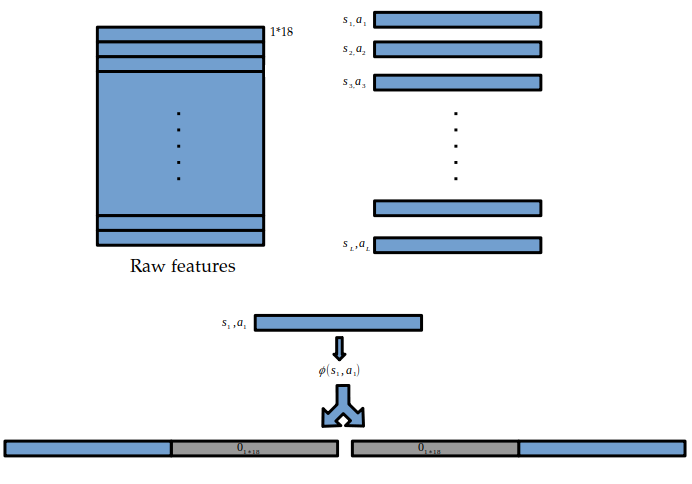
\includegraphics[scale=.40]{phi.png}
  \caption{Creating $\phi$s}
  \label{fig:phi}
\end{figure}
The following table is the Bellman Error for running different k-fold algorithms on our dataset, and train the LSPI with different folds.



\begin{center} \label{tab:be}
\begin{tabular}{ |c|c| } 
 \hline
 Method & BE \\ 
 \hline
 LSTDQ & 4935580.30 \\ 
 LSTDQ with 4-fold & 4905981.01 \\ 
 LSTDQ with 5-fold & 4601911.70 \\ 
 LSTDQ with 6-fold & 4919249.69 \\ 
 LSTDQ with 10-fold& 4886872.99 \\
 \hline
\end{tabular}
\end{center}

Based on table \ref{tab:be}, k-fold cross validation with 5 folds works quit well on our dataset.


\bibliographystyle{plain}
\bibliography{invasive_species}
\end{document}


%===============================
%========== NOT TO RUN =========
\iffalse
\section{Background} \label{sec:background}
\begin{itemize}
  \item The closest point to the span of $\Phi$ to $V^*$ is $\Pi V^*$, where $\Pi_\rho$ is the $\rho$-weighted $L_2$ projection into the span of $\Phi$.
  \[
  \Pi_\rho = \Phi (\Phi^T \Delta \Phi)^{-1} \Phi^T \Delta
  \]
\end{itemize}



\newcounter{ct}
\setcounter{ct}{1}
\whiledo {\value{ct} < 5}%
{%
  \thect\
  \stepcounter {ct}%
}



\usepackage{titlesec}

\titleformat{\section}
  {\normalfont\Large\bfseries}   % The style of the section title
  {}                             % a prefix
  {0pt}                          % How much space exists between the prefix and the title
  {Section \thesection:\quad}    % How the section is represented

% Starred variant
\titleformat{name=\section,numberless}
  {\normalfont\Large\bfseries}
  {}
  {0pt}
  {}
  

asdasd \cite{1013341}. Fig.~\ref{Fig_Example}.

{\fontfamily{pcr}\selectfont 
run files}

\begin{enumerate}
  \item The labels consists of sequential numbers.
  \item The numbers starts at 1 with every call to the enumerate environment.
\end{enumerate}

\begin{itemize}

\end{itemize}

======== HYPERLINK =============
Find the \texttt{run files} for all variants in \href{https://github.com/SHi-ON/InfoRet/tree/master/results/Assignment_4}{here}


====== FIGURES ========

\begin{figure}
	\centering
	\includegraphics[scale=.40]{Fig_Example.pdf}
	\caption{Example.}
	\label{Fig_Example}
\end{figure}

\input{second}

========= EQUATIONS =============

\begin{equation}
\left\|\frac{\partial V}{\partial\mathbf{x}_1}\right\|\left\|\mathbf{x}_1\right\|\leq c_1V\quad \text{for}\; \left\|\mathbf{x}_1\right\|\geq c_2
\end{equation}


============ TABLES =============

\begin{tabular}{ |p{3cm}|p{3cm}|p{3cm}|  }
\hline
\multicolumn{3}{|c|}{Country List} \\
\hline
Country Name     or Area Name& ISO ALPHA 2 Code &ISO ALPHA 3 \\
\hline
Afghanistan & AF &AFG \\
Aland Islands & AX   & ALA \\
Albania &AL & ALB \\
Algeria    &DZ & DZA \\
American Samoa & AS & ASM \\
Andorra & AD & AND   \\
Angola & AO & AGO \\
\hline
\end{tabular}

\begin{center}
\begin{tabular}{ |c|c|c| } 
 \hline
 cell1 & cell2 & cell3 \\ 
 cell4 & cell5 & cell6 \\ 
 cell7 & cell8 & cell9 \\ 
 \hline
\end{tabular}
\end{center}




\begin{lstlisting}[language=Python, caption=Code's name]
import numpy as np
 
def incmatrix(genl1,genl2):
    m = len(genl1)
    n = len(genl2)
    M = None #to become the incidence matrix
    VT = np.zeros((n*m,1), int)  #dummy variable
\end{lstlisting}



\begin{verbatim}
Put your codes here!
\end{verbatim}
\fi
